%%%%%%%%%%%%%%%%%%%%%%%%%%%%%%%%%%%%%%%%%%%%%%%%%%%%%%%%%%%%%%%%%%%%%%%%%%%%%%%%%%
\begin{frame}[fragile]\frametitle{}
\begin{center}
{\Large SVM}
\end{center}
\end{frame}

%%%%%%%%%%%%%%%%%%%%%%%%%%%%%%%%%%%%%%%%%%%%%%%%%%%%%%%%%%
\begin{frame}[fragile]\frametitle{Support Vector Machines (SVM)}
\begin{itemize}
\item Support vector machines are supervised machine learning algorithms that construct
separating planes for classification.
\item They are conceptually fairly simple, but the underlying mathematics for learning them from data can be tricky.
\end{itemize}
\end{frame}


%%%%%%%%%%%%%%%%%%%%%%%%%%%%%%%%%%%%%%%%%%%%%%%%%%%%%%%%%%
\begin{frame}[fragile]\frametitle{Support Vector Machines (SVM) Inventors}
\begin{itemize}
\item See video ``Vladimir Vapnik - 2012 Laureate of the Franklin Institute in Computer and Cognitive Science'' at Youtube.
\item Vladimir Vapnik discusses how his early years in Moscow helped shaped the origins of statistical learning theories, including the ideas behind the SVM. 
\item His collaborator, Isabelle Guyon, also discusses the Kernel Trick, which generalized the SVMs for non-linear decision boundaries (hence making them more popular).
\end{itemize}


\end{frame}

%%%%%%%%%%%%%%%%%%%%%%%%%%%%%%%%%%%%%%%%%%%%%%%%%%%%%%%%%
\begin{frame}[fragile]\frametitle{Support Vector Machines (SVM) Inventors}
``The invention of SVMs happened when Bernhard decided to implement Vladimir’s algorithm in the three months we had left before we moved to Berkeley. After some initial success of the linear algorithm, Vladimir suggested introducing products of features. I proposed to rather use the kernel trick of the ‘potential function’ algorithm. Vladimir initially resisted the idea because the inventors of the ‘potential functions’ algorithm (Aizerman, Braverman, and Rozonoer) were from a competing team of his institute back in the 1960’s in Russia!''
— Isabelle Guyon

\end{frame}

%%%%%%%%%%%%%%%%%%%%%%%%%%%%%%%%%%%%%%%%%%%%%%%%%%%%
\begin{frame}[fragile] \frametitle{Support vector machines Example}

\begin{itemize}
%\item It is a classification method.
\item In SVM, we plot each data item as a point in n dimensional space (where n is number of features you have) with the value of each feature being the value of
a particular coordinate.
\item For example, if we only had two features like Height and Hair length of an individual.
\item We'd first plot these two variables in two dimensional space where each point has two-coordinates.
%\item These coordinates are known as Support Vectors.
\end{itemize}
\end{frame}


%%%%%%%%%%%%%%%%%%%%%%%%%%%%%%%%%%%%%%%%%%%%%%%%%%%
\begin{frame}[fragile] \frametitle{}

\begin{center}
\includegraphics[width=0.8\linewidth]{hthair}
\end{center}
Now, we will find some line that splits the data between the two differently classified groups of
data.
\end{frame}

%%%%%%%%%%%%%%%%%%%%%%%%%%%%%%%%%%%%%%%%%%%%%%%%%%%%%%%%%%
\begin{frame}[fragile]\frametitle{Support Vector Machines (SVM)}
SVMs are the combination of two ideas
	\begin{itemize}
	\item Maximum margin classification
	\item The ``kernel trick''
	\end{itemize}
\end{frame}


%%%%%%%%%%%%%%%%%%%%%%%%%%%%%%%%%%%%%%%%%%%%%%%%%%%%%%%%%%%%%%%%%%%%%%%%%%%%%%%%%%
\begin{frame}[fragile]\frametitle{}
\begin{center}
{\Large SVM Intuition}
\end{center}
\end{frame}

%%%%%%%%%%%%%%%%%%%%%%%%%%%%%%%%%%%%%%%%%%%%%%%%%%%
\begin{frame}[fragile] \frametitle{SVM Intuition}

\begin{center}
\includegraphics[width=0.6\linewidth]{svm10}

\tiny{(Ref: How Classification Algorithms Work? - Thales Sehn Korting)}
\end{center}
\begin{itemize}
\item Suppose there are points characterized by $x_1,x_2$.
\item So these are features
\item Points are labeled with either of two classes: circles and squares.
\end{itemize}
\end{frame}



% %%%%%%%%%%%%%%%%%%%%%%%%%%%%%%%%%%%%%%%%%%%%%%%%%%%
% \begin{frame}[fragile] \frametitle{Decision Boundary}

% \begin{center}
% \includegraphics[width=0.8\linewidth]{svm6}
% \end{center}
% This will be the line such that the distances from the closest point in each of the two groups will be farthest away.
% \end{frame}

% %%%%%%%%%%%%%%%%%%%%%%%%%%%%%%%%%%%%%%%%%%%%%%%%%%%
% \begin{frame}[fragile] \frametitle{Idea: Maximize the Margin}
% The margins the distance between the decision boundary (the hyperplane) and the closest training point.
% \begin{center}
% \includegraphics[width=0.6\linewidth]{svm7}
% \end{center}
% \end{frame}

% %%%%%%%%%%%%%%%%%%%%%%%%%%%%%%%%%%%%%%%%%%%%%%%%%%%
% \begin{frame}[fragile] \frametitle{Computing the Margin}


% \begin{itemize}
% \item The tricky part will be to get an equation for the margin
% \item  We will start by getting the distance from the origin to the hyperplane
% \item 
% i.e., We want to compute the scalar $b$ below
% \end{itemize}
% \begin{center}
% \includegraphics[width=0.8\linewidth]{svm8}
% \end{center}
% \end{frame}

% %%%%%%%%%%%%%%%%%%%%%%%%%%%%%%%%%%%%%%%%%%%%%%%%%%%
% \begin{frame}[fragile] \frametitle{Computing the Margin}
% \begin{itemize}
% \item The perpendicular distance from a point $x$ to the hyperplane $w^Tx + w_0 = 0$ is $\frac{1}{||w||} | w^Tx + w_0|$
% \item The margin is the distance from the closest training point to the hyperplane $min_i\frac{1}{||w||} | w^Tx_i + w_0|$
% \end{itemize}
% \end{frame}

% %%%%%%%%%%%%%%%%%%%%%%%%%%%%%%%%%%%%%%%%%%%%%%%%%%%
% \begin{frame}[fragile] \frametitle{Support vector machines}

% \begin{itemize}
% \item The {linear}, {hard-margin} classification case can be described
% quite succinctly
% \item Pick two parallel hyperplanes that separate the two classes such
% that the distance between the hyperplanes is maximal
% \item the maximum-margin hyperplane
% is the midpoint of these two separating planes.
% \end{itemize}
% \end{frame}

% %%%%%%%%%%%%%%%%%%%%%%%%%%%%%%%%%%%%%%%%%%%%%%%%%%%
% \begin{frame}[fragile] \frametitle{}

% \begin{center}
% 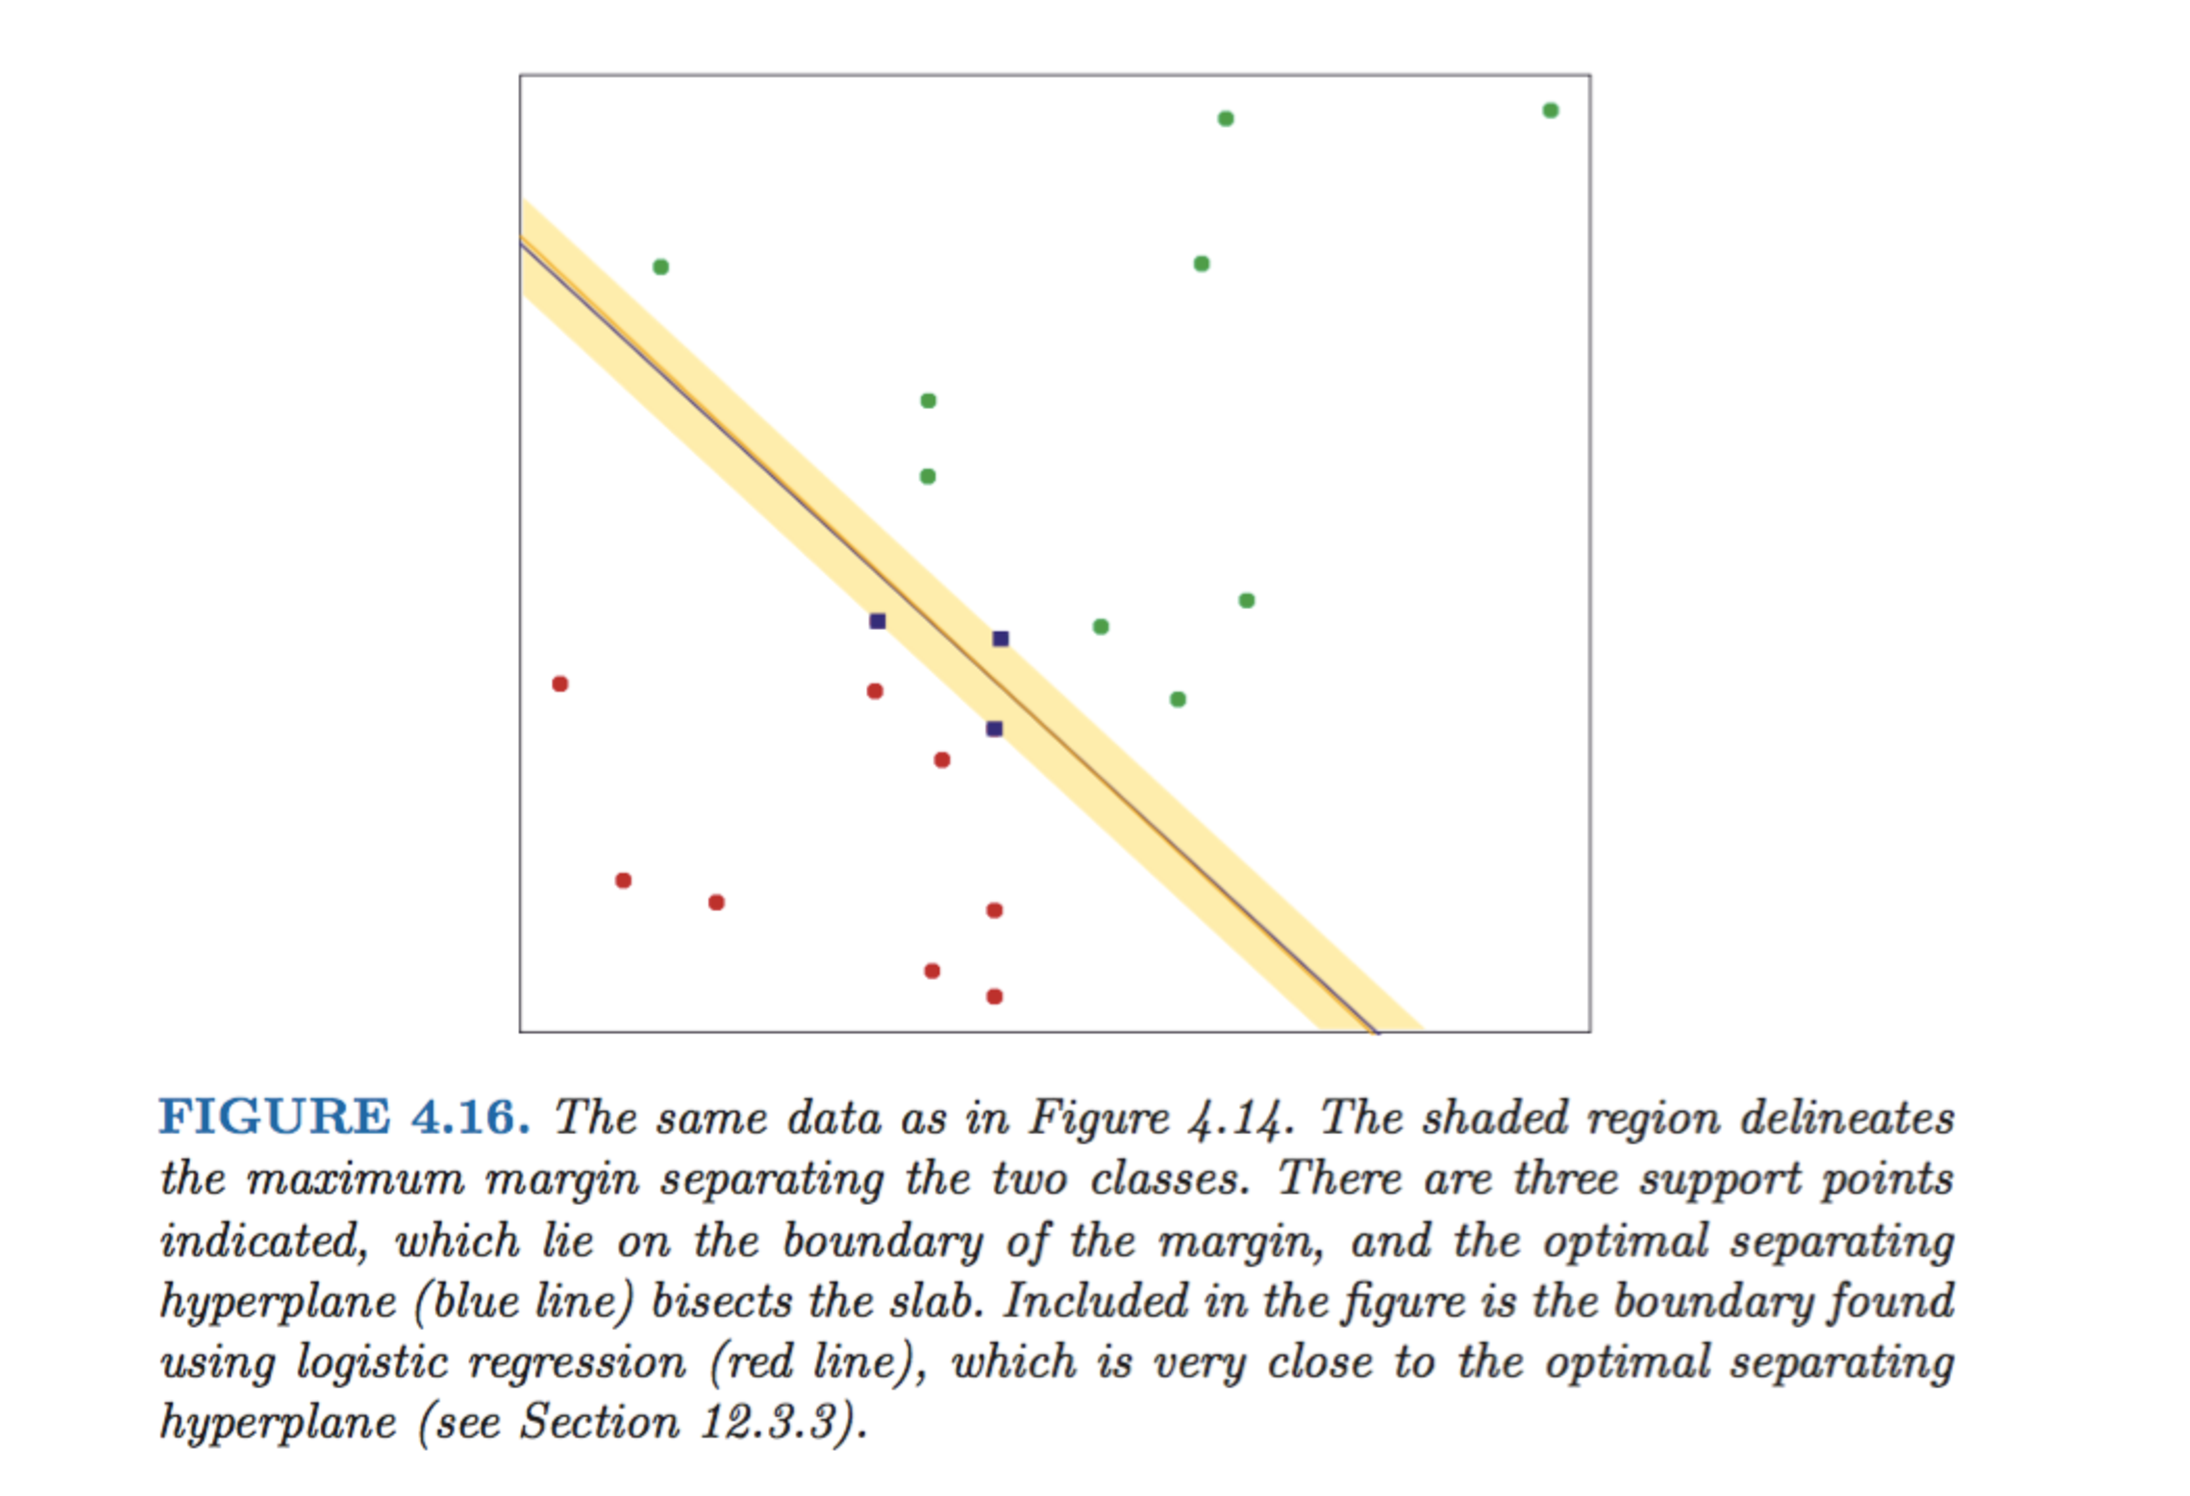
\includegraphics[width=\linewidth]{split.pdf}
% \end{center}

% \end{frame}




% %%%%%%%%%%%%%%%%%%%%%%%%%%%%%%%%%%%%%%%%%%%%%%%%%%%%%%%%%%
% \begin{frame}[fragile]\frametitle{Process}
% \begin{itemize}
% \item First, need to define a hyperplane
% \item What is a hyperplane?
% \begin{itemize}
% \item Hyperplane has p-1 dimensions in a p dimensional space
% \item Example: in 2 dimension space, a hyperplane has 1 dimension (and thus, is a line)
% \end{itemize}
% \item For two dimensions, hyperplane defined as:
% $\beta_0 + \beta_1 X_1 + \beta_2 X_2 = 0 $
% \item Its a eqn of a line.
% \item Hyperplane is dividing 2-dimesional space into two halves by a line.
% \end{itemize}
% \end{frame}

% %%%%%%%%%%%%%%%%%%%%%%%%%%%%%%%%%%%%%%%%%%%%%%%%%%%%%%%%%%
% \begin{frame}[fragile]\frametitle{Hyperplane Mathematical Definition}
% \begin{itemize}
% \item We're going to ``find'' values for $\beta_0, \beta_1, \beta_2$
% \item Then, for any values $X_1$ and $X_2$:
% \begin{itemize}
% \item If $\beta_0 + \beta_1 X_1 + \beta_2 X_2 > 0 $ then Point is not on the line. On one side of the line.
% \item If $\beta_0 + \beta_1 X_1 + \beta_2 X_2 < 0 $ then Point is not on the line. On another side of the line.
% \end{itemize}

% \end{itemize}

% \adjustbox{valign=t}{
% \begin{minipage}{0.45\linewidth}
% \begin{center}
% \includegraphics[width=0.8\linewidth,keepaspectratio]{hyp}
% \end{center}
% \end{minipage}
% }
% \hfill
% \adjustbox{valign=t}{
% \begin{minipage}{0.45\linewidth}
% For a new test instance, which side of the line is it on?

% \begin{itemize}
% \item $\beta_0 + \beta_1 X_1 + \beta_2 X_2 > 0 $ 
% \item $\beta_0 + \beta_1 X_1 + \beta_2 X_2 < 0 $ 
% \end{itemize}

% \end{minipage}
% }
% \end{frame}




%%%%%%%%%%%%%%%%%%%%%%%%%%%%%%%%%%%%%%%%%%%%%%%%%%%
\begin{frame}[fragile] \frametitle{SVM Intuition}

\begin{center}
\includegraphics[width=0.6\linewidth]{svm11}

\tiny{(Ref: How Classification Algorithms Work? - Thales Sehn Korting)}
\end{center}
\begin{itemize}
\item Goal is to find a separating plane that separates the classes as per the training data
\item Generic Hyper-plane's equation is taken as $g(\overrightarrow{x}) = \overrightarrow{w}^T \overrightarrow{x}+ w_0$
\end{itemize}
\end{frame}



%%%%%%%%%%%%%%%%%%%%%%%%%%%%%%%%%%%%%%%%%%%%%%%%%%%
\begin{frame}[fragile] \frametitle{SVM Intuition}

\begin{center}
\includegraphics[width=0.6\linewidth]{svm12}

\tiny{(Ref: How Classification Algorithms Work? - Thales Sehn Korting)}
\end{center}
\begin{itemize}
\item Many Hyper-planes can classify the data correctly.
\item But which one is the best?
\end{itemize}
\end{frame}

%%%%%%%%%%%%%%%%%%%%%%%%%%%%%%%%%%%%%%%%%%%%%%%%%%%
\begin{frame}[fragile] \frametitle{SVM Intuition}

\begin{center}
\includegraphics[width=0.6\linewidth]{svm13}
\end{center}
\begin{itemize}
\item The one with Maximum margin is the best.
\item $Z_2$ is better than $Z_1$, so nice and distinct separation.
\end{itemize}
\end{frame}

%%%%%%%%%%%%%%%%%%%%%%%%%%%%%%%%%%%%%%%%%%%%%%%%%%%
\begin{frame}[fragile] \frametitle{SVM Intuition}

\begin{center}
\includegraphics[width=0.6\linewidth]{svm14}

\tiny{(Ref: How Classification Algorithms Work? - Thales Sehn Korting)}
\end{center}
\begin{itemize}
\item For data points labeled as circles, when features are put into ``g'' equation, the result is more than equal to 1
\item For data points labeled as squares, when features are put into ``g'' equation, the result is less than equal to -1
\end{itemize}
\end{frame}

%%%%%%%%%%%%%%%%%%%%%%%%%%%%%%%%%%%%%%%%%%%%%%%%%%%%%%%%%%%%%%%%%%%%%%%%%%%%%%%%%%
\begin{frame}[fragile]\frametitle{}
\begin{center}
{\Large SVM Quick Derivation}
\end{center}
\end{frame}

%%%%%%%%%%%%%%%%%%%%%%%%%%%%%%%%%%%%%%%%%%%%%%%%%%%
\begin{frame}[fragile] \frametitle{Which is the best line?}
\begin{center}
\includegraphics[width=0.8\linewidth]{svm23}

\tiny{(Ref: Support Vector Machine - Georgia Tech - Machine Learning - Udacity)}
\end{center}


\begin{itemize}
\item Question: Which is the best line?
\item Not any random line!!
\item There are 3 green dots and 3 red dots in the gap (gutter/margin), which 2 dots form best line?
\end{itemize}
\end{frame}

%%%%%%%%%%%%%%%%%%%%%%%%%%%%%%%%%%%%%%%%%%%%%%%%%%%
\begin{frame}[fragile] \frametitle{Better Margin for Unseen points}
\begin{center}
\includegraphics[width=0.8\linewidth]{svm24}

\tiny{(Ref: Support Vector Machine - Georgia Tech - Machine Learning - Udacity)}
\end{center}


\begin{itemize}
\item With 3 green forming lines with 3 reds each, there are 9 possible lines.
\item And the ALL separate the positive and negative points.
\item Intuitively, we thought that the middle line looks GOOD.
\item The second, more slanting line is not good as its closer to some of the points than the middle line. Like Over-fitting.
\item We need clear and BIG separation to avoid mis-classifications as much as possible. Because we don't know what un-seen points will bring. Better the gutter, better chances of good classification.
\end{itemize}
\end{frame}


%%%%%%%%%%%%%%%%%%%%%%%%%%%%%%%%%%%%%%%%%%%%%%%%%%%
\begin{frame}[fragile] \frametitle{Maximum Margin}
\begin{center}
\includegraphics[width=0.8\linewidth]{svm22}

\tiny{(Ref: Support Vector Machine - Georgia Tech - Machine Learning - Udacity)}
\end{center}


\begin{itemize}
\item Even for parallel lines, the side lines are not good as they are CLOSE to either of the positive or negative lines.
\item Top line is where the closest Positive line, bottom is to Negative line. 
\item Middle is the best as it has good space/margin around it.
\item So, Goal is to find a separating plane that separates the classes as per the training data
\end{itemize}
\end{frame}


%%%%%%%%%%%%%%%%%%%%%%%%%%%%%%%%%%%%%%%%%%%%%%%%%%%
\begin{frame}[fragile] \frametitle{Hperplane with Boolean output}
\begin{center}
\includegraphics[width=0.8\linewidth]{svm25}

\tiny{(Ref: Support Vector Machine - Georgia Tech - Machine Learning - Udacity)}
\end{center}

Maths revision: Equations:
\begin{itemize}
\item Equation of line is $y = mx + b$.  If $x$ has more than 2 dimensions, then this is equation of a plane, a hyper plane and then $mx$ changes to $w^TX$, where $w$ is slopes vector.
\item Here $y$ is not the coordinate, but boolean values.
\end{itemize}
\end{frame}

%%%%%%%%%%%%%%%%%%%%%%%%%%%%%%%%%%%%%%%%%%%%%%%%%%%
\begin{frame}[fragile] \frametitle{Middle Hyperplane}
\begin{center}
\includegraphics[width=0.8\linewidth]{svm26}

\tiny{(Ref: Support Vector Machine - Georgia Tech - Machine Learning - Udacity)}
\end{center}

Maths revision: Equations:
\begin{itemize}
\item $y$ : classification label
\item $w^T$ : parameters, weights, coefficients
\item $b$ : bias
\item Question: What would be output $y$ for any point ($x$) on the middle line?
\end{itemize}
\end{frame}

%%%%%%%%%%%%%%%%%%%%%%%%%%%%%%%%%%%%%%%%%%%%%%%%%%%
\begin{frame}[fragile] \frametitle{SVM Derivation}
\begin{center}
\includegraphics[width=0.8\linewidth]{svm27}

\tiny{(Ref: Support Vector Machine - Georgia Tech - Machine Learning - Udacity)}
\end{center}

\begin{itemize}
\item 0. As its neither positive nor negative.
\item  So, the equation of the middle line is $w^TX + b = 0$
\item What are the equations of other boundary lines?
\item So, lets make them $-1$ and $+1$, to denote negative and positive labels.
\end{itemize}
\end{frame}


%%%%%%%%%%%%%%%%%%%%%%%%%%%%%%%%%%%%%%%%%%%%%%%%%%%
\begin{frame}[fragile] \frametitle{SVM Derivation}
\begin{center}
\includegraphics[width=0.8\linewidth]{svm21}

\tiny{(Ref: Support Vector Machine - Georgia Tech - Machine Learning - Udacity)}
\end{center}

\begin{itemize}
\item On the line $y=0$ so eqn of the hyperplane is  $\overrightarrow{w}^T \overrightarrow{x}+ b = 0$
\item For left support point, $y=-1$ so equation of left support boundary is  $\overrightarrow{w}^T \overrightarrow{x}+ b = -1$ And the full zone as $\leq -1$
\item For right support point, $y=+1$ so equation of right support boundary is  $\overrightarrow{w}^T \overrightarrow{x}+ b = +1$ And the full zone as $\geq +1$
%\item Its $b$ away from the origin.
%\item Generically, it is $g(\overrightarrow{x}) = \overrightarrow{w}^T \overrightarrow{x}+ w_0$
\end{itemize}
\end{frame}

%%%%%%%%%%%%%%%%%%%%%%%%%%%%%%%%%%%%%%%%%%%%%%%%%%%
\begin{frame}[fragile] \frametitle{SVM Derivation}
\begin{center}
\includegraphics[width=0.8\linewidth]{svm28}

\tiny{(Ref: Support Vector Machine - Georgia Tech - Machine Learning - Udacity)}
\end{center}

\begin{itemize}
\item We want Margin/Width to be maximum. What is the equation of the Width?
\item Can we find out, as the Width line is perpendicular to, to the boundary lines and its made of end points lying on the boundary lines?
\item Lets call the points $x_1$ and $x_2$, so the vector diff between these is Width.
\end{itemize}
\end{frame}

%%%%%%%%%%%%%%%%%%%%%%%%%%%%%%%%%%%%%%%%%%%%%%%%%%%
\begin{frame}[fragile] \frametitle{Equation of Width}
\begin{center}
\includegraphics[width=\linewidth]{svm29}

\tiny{(Ref: Support Vector Machine - Georgia Tech - Machine Learning - Udacity)}
\end{center}

\begin{itemize}
\item Two equations, 2 unknowns. Subtract. Result is $w^T(x_1 - x_2) = 2$
\item Assume $w$ is a number , you would divide 2 by it. But it is a vector. Why not take divide each side by length of $w$. $w/||w||$ is unit vector.
\item So, on left hand side: $x_1 - x_2$ vector has been projected on unit $w$ vector. Thats dot product, which is 2.
\end{itemize}
\end{frame}

%%%%%%%%%%%%%%%%%%%%%%%%%%%%%%%%%%%%%%%%%%%%%%%%%%%
\begin{frame}[fragile] \frametitle{Maximizing Width}
\begin{center}
\includegraphics[width=0.8\linewidth]{svm30}

\tiny{(Ref: Support Vector Machine - Georgia Tech - Machine Learning - Udacity)}
\end{center}

\begin{itemize}
\item $w$ is the direction along perpendicular to boundary lines, the width direction.
\item So, we maximize width $m$ (``margin'') while classifying everything correctly (thats the constraint)
\item But how to put this constraint mathematically?
\end{itemize}
\end{frame}

%%%%%%%%%%%%%%%%%%%%%%%%%%%%%%%%%%%%%%%%%%%%%%%%%%%
\begin{frame}[fragile] \frametitle{Combining 2 Equations}
\begin{center}
\includegraphics[width=0.8\linewidth]{svm31}

\tiny{(Ref: Support Vector Machine - Georgia Tech - Machine Learning - Udacity)}
\end{center}

\begin{itemize}
\item Lets combine both boundary lines equations into one, by leveraging the label $y_i$ itself.
\item $y_i(w^TX_i + b) \ge 1$. The ``plus minus 1'' thing on the right side has changed to just ``plus 1'' because $y_i$ becomes minus if right hand side is minus, and both cancel out!!! Wonderful trick.
\end{itemize}
\end{frame}

%%%%%%%%%%%%%%%%%%%%%%%%%%%%%%%%%%%%%%%%%%%%%%%%%%%
\begin{frame}[fragile] \frametitle{Hard Stuff, Leap of Faith}
\begin{center}
\includegraphics[width=0.8\linewidth]{svm32}

\tiny{(Ref: Support Vector Machine - Georgia Tech - Machine Learning - Udacity)}
\end{center}

\begin{itemize}
\item Instead of solving ``max $\frac{2}{||w||}$ problem, is better to solve ``min $\frac{1}{2}||w||^2$'' problem. (Because lengths are positive and now we get good convex function to optimize, easier to compute by algorithm. Its a quadratic programming problem, and people know how to solve it. It has unique solution. )
\item Another (not to be questioned!!) change is to convert the quadratic programming eqn to maximizing Lagrange Multiplier optimization form.
\item Its sum of alphas (for all i data points) minus half time, every pair points, x and label(y) values, multiplied by own alphas; with constraints such as alphas are positives and the other constraint shown.
\end{itemize}
\end{frame}

%%%%%%%%%%%%%%%%%%%%%%%%%%%%%%%%%%%%%%%%%%%%%%%%%%%
\begin{frame}[fragile] \frametitle{Just assume, This Works!!}
\begin{center}
\includegraphics[width=0.8\linewidth]{svm33}

\tiny{(Ref: Support Vector Machine - Georgia Tech - Machine Learning - Udacity)}
\end{center}

Properties:
\begin{itemize}
\item Maximizing alphas, then $W$ can be calculated the $b$ can be calculated.
\item Lets make small $w$ is the 2nd term.
\item Most of the alphas are 0. Means only few points are part of the summation. The points for which alphas are non-zero are called support vectors. They are the points on the boundary lines.
\item So, this is the Machine that needs only Support Vectors.
\end{itemize}
\end{frame}

%%%%%%%%%%%%%%%%%%%%%%%%%%%%%%%%%%%%%%%%%%%%%%%%%%%
\begin{frame}[fragile] \frametitle{SVM Derivation Closure}
\begin{center}
\includegraphics[width=0.8\linewidth]{svm34}

\tiny{(Ref: Support Vector Machine - Georgia Tech - Machine Learning - Udacity)}
\end{center}

Properties:
\begin{itemize}
\item Points away DO NOT MATTER. Its like Nearest Neighbor where only local points matter!! But here K is not provided, but we already know support points (and thus their count, ie K) by quadratic programing
\item The x product terms, are the dot products. If both are in same line, its a large number, but if they are perpendicular its towards 0. Its similarity.
\item So, find all support points, and from that keep only collinear like points.
\item This maximizes W, and thus the width.
\end{itemize}
\end{frame}


%%%%%%%%%%%%%%%%%%%%%%%%%%%%%%%%%%%%%%%%%%%%%%%%%%%%%%%%%%%%%%%%%%%%%%%%%%%%%%%%%%
\begin{frame}[fragile]\frametitle{}
\begin{center}
{\Large Back to SVM Intuition, old symbols}
\end{center}
\end{frame}


%%%%%%%%%%%%%%%%%%%%%%%%%%%%%%%%%%%%%%%%%%%%%%%%%%%
\begin{frame}[fragile] \frametitle{SVM Intuition}

\begin{center}
\includegraphics[width=0.6\linewidth]{svm15}

\tiny{(Ref: How Classification Algorithms Work? - Thales Sehn Korting)}
\end{center}
\begin{itemize}
\item Distance of a point from a hyper-plane is $z$
\item Given by a formula $z = \frac{|g(x)|}{||w||}$, is also called `margin'
\end{itemize}
\end{frame}

%%%%%%%%%%%%%%%%%%%%%%%%%%%%%%%%%%%%%%%%%%%%%%%%%%%
\begin{frame}[fragile] \frametitle{SVM Intuition}

\begin{center}
\includegraphics[width=0.6\linewidth]{svm16}

\tiny{(Ref: How Classification Algorithms Work? - Thales Sehn Korting)}
\end{center}
\begin{itemize}
\item For any point, $g(\overrightarrow{x})$ is atleast ``1'', on either side (this is the minimum-est, g(x) can get, from the formula)
\item So min distance on either side is $\frac{1}{||\overrightarrow{w}||}$
\item Total margin from both sides is $\frac{2}{||\overrightarrow{w}||}$
\item So, if we minimize $\overrightarrow{w}$, then margin will be maximum.
\end{itemize}
\end{frame}

% %%%%%%%%%%%%%%%%%%%%%%%%%%%%%%%%%%%%%%%%%%%%%%%%%%%
% \begin{frame}[fragile] \frametitle{SVM Intuition}

% \begin{center}
% \includegraphics[width=0.6\linewidth]{svm17}

% \tiny{(Ref: How Classification Algorithms Work? - Thales Sehn Korting)}
% \end{center}
% \begin{itemize}
% \item Optimization for weights is non-trivial
% \end{itemize}
% \end{frame}

%%%%%%%%%%%%%%%%%%%%%%%%%%%%%%%%%%%%%%%%%%%%%%%%%%%%%%%%%%%%%%%%%%%%%%%%%%%%%%%%%%
\begin{frame}[fragile]\frametitle{}
\begin{center}
{\Large SVM Example}
\end{center}
\end{frame}

%%%%%%%%%%%%%%%%%%%%%%%%%%%%%%%%%%%%%%%%%%%%%%%%%%%
\begin{frame}[fragile] \frametitle{SVM Example}

\begin{center}
\includegraphics[width=0.6\linewidth]{svm18}

\tiny{(Ref: How Classification Algorithms Work? - Thales Sehn Korting)}
\end{center}
\begin{itemize}
\item Lets say we have just 3 points, 2 circles ([1,1] and [2,0]) and one square [2,3]
\item We want to design SVM classifier, ie the Hyper-plane
\end{itemize}
\end{frame}

%%%%%%%%%%%%%%%%%%%%%%%%%%%%%%%%%%%%%%%%%%%%%%%%%%%
\begin{frame}[fragile] \frametitle{SVM Example}

\begin{center}
\includegraphics[width=0.5\linewidth]{svm19}

\tiny{(Ref: How Classification Algorithms Work? - Thales Sehn Korting)}
\end{center}
\begin{itemize}
\item We know that the hyper-plane line would be equidistant from two closest points (2,3) and (1,1)
\item So, generically the weight vector would be of the form $ \bar{w} = (2,3) - (1,1) = (a,2a)$
\item Need to find $a$ and then $\bar{w}, w_0$
\end{itemize}
\end{frame}

%%%%%%%%%%%%%%%%%%%%%%%%%%%%%%%%%%%%%%%%%%%%%%%%%%%
\begin{frame}[fragile] \frametitle{SVM Example}
\begin{itemize}
\item weight vector $\bar{w} = (a,2a)$
\item Using Negative point (1,1), putting in equation $g(\bar{x}) = \bar{w}x + w_0 = y$ is $g(1,1) = (a,2a).(1,1) + w_0 = -1$, is $a + 2a + w_0 = -1$
\item Using Positive point (2,3), putting in equation $g(\bar{x}) = \bar{w}x + w_0 = y$ is $g(2,3) = (a,2a).(2,3) + w_0 = 1$, is $2a + 6a + w_0 = 1$
\item Solving these two equations simultaneously. From 1st, $w_0 = 1 - 8a$. Putting it in 2nd $3a + 1 - 8a = -1$, thus $5a = 2$ so $a = \frac{2}{5}$
\item Putting $a$ in the first equation, $ w_0 = 1 - 8\frac{2}{5} = \frac{11}{5}$
\item Thus , $ \bar{x} = (\frac{2}{5},\frac{4}{5})$
\item Putting in original Hyperplane equation $g(\bar{x}) = \frac{2}{5}x_1 + \frac{4}{5}x_2 - \frac{11}{5}$
\item Being equal to 0 for the middle line, it can be simplified to $g(\bar{x}) = x_1 + 2x_2 - 5.5$
\end{itemize}
\end{frame}


%%%%%%%%%%%%%%%%%%%%%%%%%%%%%%%%%%%%%%%%%%%%%%%%%%%
\begin{frame}[fragile] \frametitle{SVM Example}
\begin{center}
\includegraphics[width=0.8\linewidth]{svm20}

\tiny{(Ref: How Classification Algorithms Work? - Thales Sehn Korting)}
\end{center}
\end{frame}


%%%%%%%%%%%%%%%%%%%%%%%%%%%%%%%%%%%%%%%%%%%%%%%%%%%%%%%%%%%%%%%%%%%%%%%%%%%%%%%%%%
\begin{frame}[fragile]\frametitle{}
\begin{center}
{\Large SVM Aspects}
\end{center}
\end{frame}

% %%%%%%%%%%%%%%%%%%%%%%%%%%%%%%%%%%%%%%%%%%%%%%%%%%%%%%%%%%
% \begin{frame}[fragile]\frametitle{Classification}
% Standard SVM approach:

% \begin{itemize}
% \item Label class data as either +1 or -1, depending on which class an instance belongs to.
% \item Prediction:

% \begin{center}
% \includegraphics[width=0.8\linewidth,keepaspectratio]{hypeqn}
% \end{center}

% \item Can also look at the magnitude: How far from zero?
% Greater magnitude means more confident prediction.
% \item This is not a Gradient Descent like minimization problem, but an maximization-optimization problem.
% \item Maximizing distance, ie margin.
% \end{itemize}
% \end{frame}

% %%%%%%%%%%%%%%%%%%%%%%%%%%%%%%%%%%%%%%%%%%%%%%%%%%%
% \begin{frame}[fragile] \frametitle{Maximum Margin Hyper-plane}
% What's the best separating hyperplane?
% %\adjustbox{valign=t}{
% %\begin{minipage}{0.45\linewidth}
% \begin{center}
% \includegraphics[width=0.45\linewidth,keepaspectratio]{marg}
% \end{center}
% %\end{minipage}
% %}
% %\hfill
% %\adjustbox{valign=t}{
% %\begin{minipage}{0.45\linewidth}

% \begin{itemize}
% \item $B_1$ and $B_2$ are each separating hyperplanes. $B_1$ is better
% %\item Margin: the smallest distance from the hyperplane to the training data
% %\item We want the hyperplane that has the greatest margin.
% \item Support Vectors: the points in the data, that if moved, the maximal margin hyper-plane would move as well
% \item Moving any of the other data points would not affect the model.
% \end{itemize}
% %\end{minipage}
% %}
% \end{frame}
% %
% %%%%%%%%%%%%%%%%%%%%%%%%%%%%%%%%%%%%%%%%%%%%%%%%%%%%
% %\begin{frame}[fragile] \frametitle{Maximum Margin Hyperplane}
% %What's the best separating hyperplane?
% %%\adjustbox{valign=t}{
% %%\begin{minipage}{0.45\linewidth}
% %\begin{center}
% %\includegraphics[width=0.45\linewidth,keepaspectratio]{marg1}
% %\end{center}
% %%\end{minipage}
% %%}
% %%\hfill
% %%\adjustbox{valign=t}{
% %%\begin{minipage}{0.45\linewidth}
% %
% %\begin{itemize}
% %
% %
% %\end{itemize}
% %%\end{minipage}
% %%}
% %\end{frame}

%%%%%%%%%%%%%%%%%%%%%%%%%%%%%%%%%%%%%%%%%%%%%%%%%%%%%%%%%%
\begin{frame}[fragile]\frametitle{New point added }
\begin{center}
\includegraphics[width=\linewidth,keepaspectratio]{newptsvm}
\end{center}
\end{frame}




%%%%%%%%%%%%%%%%%%%%%%%%%%%%%%%%%%%%%%%%%%%%%%%%%%%%%%%%%%
\begin{frame}[fragile]\frametitle{Constructing the Support Vector Classifier }
\begin{itemize}
\item How much ``softness'' (mis-classifications) is ideal?
\item Specification of non-negative tuning parameter C
\begin{itemize}
\item Generally chosen by analyst following cross-validation
\item Large C: wider margin; more instances violate margin
\item Small C: narrower margin; less tolerance for instances that violate margin
\end{itemize}
\end{itemize}
\begin{center}
\includegraphics[width=0.8\linewidth,keepaspectratio]{csvm}
\end{center}
\end{frame}


%%%%%%%%%%%%%%%%%%%%%%%%%%%%%%%%%%%%%%%%%%%%%%%%%%%%%%%%%%
\begin{frame}[fragile]\frametitle{Non-linear decision boundary?}
What if a non-linear decision boundary is needed?
\begin{center}
\includegraphics[width=0.8\linewidth,keepaspectratio]{nlsvm}
\end{center}
Poor performance using this decision boundary.
Can we twist the boundary? Or
Can we twist the data?
\end{frame}

%%%%%%%%%%%%%%%%%%%%%%%%%%%%%%%%%%%%%%%%%%%%%%%%%%%
\begin{frame}[fragile] \frametitle{Non-linear Dataset}

Non-linear data set are difficult to be separated using a linear hyperplane. SVM algorithm is related to finding the hyperplane which separates the data based on maximum margin. 

E.g. Iris dataset

\begin{center}
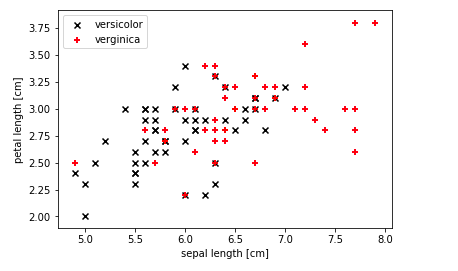
\includegraphics[width=0.5\linewidth]{svm38}

\end{center}

The above data set is in 2-dimensions. And, it is not linearly inseparable in a smooth manner.

{\tiny (Ref: Machine Learning – SVM Kernel Trick Example - Ajitesh Kumar)}
\end{frame}


%%%%%%%%%%%%%%%%%%%%%%%%%%%%%%%%%%%%%%%%%%%%%%%%%%%
\begin{frame}[fragile] \frametitle{Non-linear Dataset}

Can the data set be represented in the following form by adding another dimension? If it is possible, a hyperplane can be found which separates them clearly.

\begin{center}
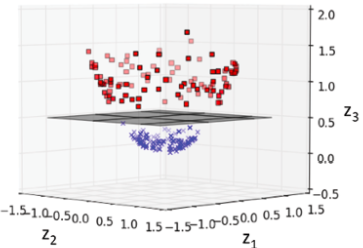
\includegraphics[width=0.5\linewidth]{svm39}

\end{center}

This is where the kernel method comes to the rescue. The idea is to apply a function that projects / transform the data in such a manner that the data becomes linearly separable. In case of SVM algorithm, data becomes linearly separable by applying maximum margin.

{\tiny (Ref: Machine Learning – SVM Kernel Trick Example - Ajitesh Kumar)}
\end{frame}

%%%%%%%%%%%%%%%%%%%%%%%%%%%%%%%%%%%%%%%%%%%%%%%%%%%
\begin{frame}[fragile] \frametitle{Simple Example}

1-D: not easy to separate and how adding another dimension makes it easy.

\begin{center}
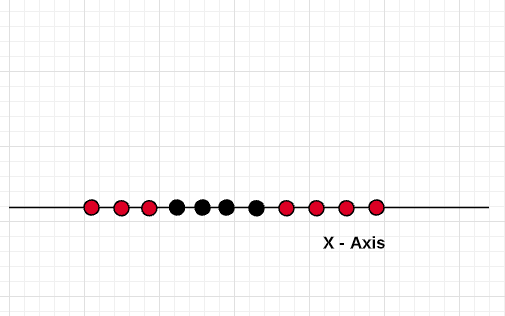
\includegraphics[width=0.6\linewidth]{svm40}

\end{center}

{\tiny (Ref: Machine Learning – SVM Kernel Trick Example - Ajitesh Kumar)}
\end{frame}

%%%%%%%%%%%%%%%%%%%%%%%%%%%%%%%%%%%%%%%%%%%%%%%%%%%
\begin{frame}[fragile] \frametitle{Simple Example}

Let’s apply the method of adding another dimension to the data by using the function $Y = X^2$ (X-squared). Thus, the data looks like the following after applying the kernel function ($Y = X^2$) and becomes linearly separable.
\begin{center}
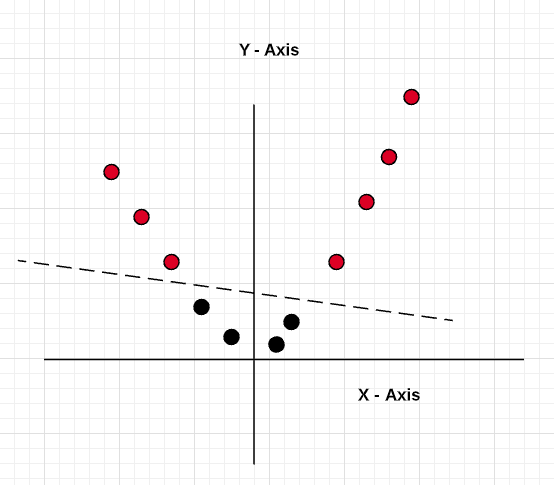
\includegraphics[width=0.6\linewidth]{svm41}

\end{center}

{\tiny (Ref: Machine Learning – SVM Kernel Trick Example - Ajitesh Kumar)}
\end{frame}

%%%%%%%%%%%%%%%%%%%%%%%%%%%%%%%%%%%%%%%%%%%%%%%%%%%
\begin{frame}[fragile] \frametitle{What are Kernel Methods?}

\begin{itemize}
\item The idea is to create nonlinear combinations of the original features to project them onto a higher-dimensional space via a mapping function, , where the data becomes linearly separable. 
\item In the diagram given below, the two-dimensional dataset (X1, X2) is projected into a new three-dimensional feature space (Z1, Z2, Z3) where the classes become separable.
\end{itemize}


\begin{center}
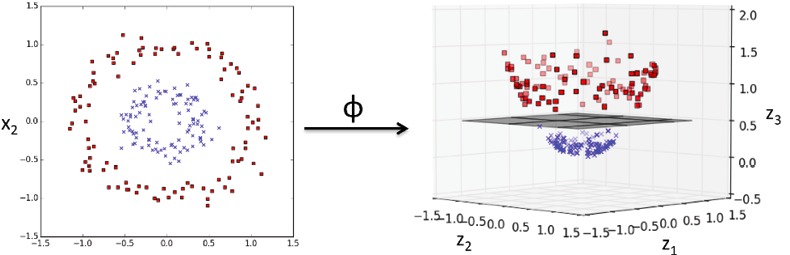
\includegraphics[width=0.8\linewidth]{svm42}

\end{center}

{\tiny (Ref: Machine Learning – SVM Kernel Trick Example - Ajitesh Kumar)}
\end{frame}


%%%%%%%%%%%%%%%%%%%%%%%%%%%%%%%%%%%%%%%%%%%%%%%%%%%
\begin{frame}[fragile] \frametitle{What are Kernel Methods?}

\begin{itemize}
\item Kernel trick is to convert dot product of support vectors to the dot product of mapping function. 
\item Recall the optimization problem for SVM:

\begin{center}
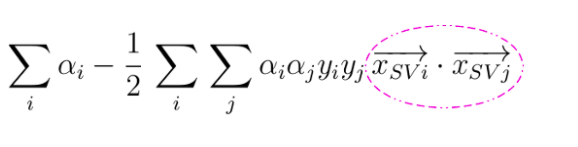
\includegraphics[width=0.6\linewidth]{svm43}

\end{center}

\item Pay attention to the pink circle which represents the dot product of the support vectors. The trick is to replace this inner product with another one without even knowing $\phi$

\begin{center}
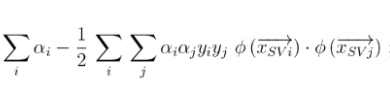
\includegraphics[width=0.6\linewidth]{svm44}

\end{center}

\item From above, if there is a function that can be represented as an inner product of mapping function, all we will be required to know is that function and not the mapping function. That function is called a Kernel Function.
\end{itemize}




{\tiny (Ref: Machine Learning – SVM Kernel Trick Example - Ajitesh Kumar)}
\end{frame}

%%%%%%%%%%%%%%%%%%%%%%%%%%%%%%%%%%%%%%%%%%%%%%%%%%%
\begin{frame}[fragile] \frametitle{What are Kernel Functions and its different types?}

\begin{itemize}
\item The kernel function is a function which can be represented the dot product of the mapping function (kernel method) and can be represented as the following:

\begin{center}
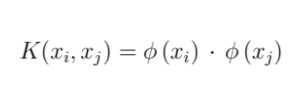
\includegraphics[width=0.4\linewidth]{svm45}

\end{center}

\item Kernel function reduces the complexity of finding the mapping function. So, the kernel function defines the inner product in the transformed space. The following are different kinds of kernel functions. 

\begin{itemize}

\item Polynomial kernel
\item Gaussian kernel
\item Radial basis function (RBF) kernel
\item Sigmoid kernel
\end{itemize}
\end{itemize}




{\tiny (Ref: Machine Learning – SVM Kernel Trick Example - Ajitesh Kumar)}
\end{frame}



% %%%%%%%%%%%%%%%%%%%%%%%%%%%%%%%%%%%%%%%%%%%%%%%%%%%
% \begin{frame}[fragile] \frametitle{Circle Transformations}
% \begin{center}
% \includegraphics[width=0.8\linewidth]{svm35}

% \tiny{(Ref: Support Vector Machine - Georgia Tech - Machine Learning - Udacity)}
% \end{center}

% \begin{itemize}
% \item Each data point is transformed into another space, with multiple value tuple
% \item Not changing original data, but creating new features (temporarily) for classification
% \item In Quadratic optimization problem, the $x_i^Tx_j$ term, is turned into the tuple. So, for points
% like $(x_1,y_1), (x_2,y_2)$ the tuple becomes, for x vector $x_1^2,x_2^2,\sqrt{2}x_1x_2$ and for y vector $y_1^2,y_2^2,\sqrt{2}y_1y_2$
% \end{itemize}
% \end{frame}

% %%%%%%%%%%%%%%%%%%%%%%%%%%%%%%%%%%%%%%%%%%%%%%%%%%%
% \begin{frame}[fragile] \frametitle{Circle Transformations}
% \begin{center}
% \includegraphics[width=0.8\linewidth]{svm35}

% \tiny{(Ref: Support Vector Machine - Georgia Tech - Machine Learning - Udacity)}
% \end{center}

% \begin{itemize}
% \item Dot product of both vectors is: $x_1^2y_1^2+2x_1x_2y_1y_2+x_2^2y_2^2$, remember anything?
% \item Factorize $x_1^2y_1^2+2x_1x_2y_1y_2+x_2^2y_2^2$ to get $(x_1y_1+x_2y_2)^2$, its actually $(X^Ty)^2$
% \item Does that mean the dot product got transformed into dot product's square? Made a circle.
% \end{itemize}
% \end{frame}


% %%%%%%%%%%%%%%%%%%%%%%%%%%%%%%%%%%%%%%%%%%%%%%%%%%%
% \begin{frame}[fragile] \frametitle{Circle Transformations}
% \begin{center}
% \includegraphics[width=0.8\linewidth]{svm36}

% \tiny{(Ref: Support Vector Machine - Georgia Tech - Machine Learning - Udacity)}
% \end{center}

% \begin{itemize}
% \item From 2D to 3D (tuple), the pluses have got above, the minuses have gone below, and thus we can have a separating Hyperplane
% \item Now we can have Circular Boundary of separation, and can be seen projection.
% \item Actually we don't need to form tuple, just square the dot product term, and then do quadratic programing, then its able to separate. That happens when you say ``rbf'' kernel in place of ``linear'' kernel.
% \end{itemize}
% \end{frame}

% %%%%%%%%%%%%%%%%%%%%%%%%%%%%%%%%%%%%%%%%%%%%%%%%%%%
% \begin{frame}[fragile] \frametitle{Circle Transformations}
% \begin{center}
% \includegraphics[width=0.8\linewidth]{svm37}

% \tiny{(Ref: Support Vector Machine - Georgia Tech - Machine Learning - Udacity)}
% \end{center}

% \begin{itemize}
% \item Lets call the kernel as function $K()$, its still a notion of similarity.
% \item Projecting in higher dimensional space then do linear separation.
% \item Many kernels are possible.
% \item (Mine: Please note that the y shown here is not a label, but the data points x and y.)
% \item The kernel functions have to follow the ``Mercer Condition'' (not to be discussed!!, its well behaved distance function.)
% \end{itemize}
% \end{frame}



% %%%%%%%%%%%%%%%%%%%%%%%%%%%%%%%%%%%%%%%%%%%%%%%%%%%%%%%%%%
% \begin{frame}[fragile]\frametitle{Kernel Tricks: Data Transformation}
% \begin{center}
% \includegraphics[width=\linewidth,keepaspectratio]{attrsvm}
% \end{center}
% Even adding a third dimension and then separating 2D points in 3D is possible.
% \tiny{(Reference: Introduction to Machine Learning - Jeff Howbert)}
% \end{frame}
%
%%%%%%%%%%%%%%%%%%%%%%%%%%%%%%%%%%%%%%%%%%%%%%%%%%%%%%%%%%%
%\begin{frame}[fragile]\frametitle{Some Concerns }
%\begin{itemize}
%\item What's the best separating hyperplane?
%
%\item What if a ``separting hyperplane'' can't be formed
%\item Data is more than two dimensions
%\item Regression instead of classification
%\end{itemize}
%SVMs can deal with each of these.
%\end{frame}
%
%%%%%%%%%%%%%%%%%%%%%%%%%%%%%%%%%%%%%%%%%%%%%%%%%%%%%%%%%%%
%\begin{frame}[fragile]\frametitle{Other extensions to SVMs}
%
%\begin{itemize}
%\item Nonlinear SVM Model
%\item Regression instead of classification
%\item Categorical variables instead of continuous
%\item Multiclass problems instead of binary
%\item Radial ``kernals''. Circle instead of hyperplane
%\end{itemize}
%\end{frame}

%%%%%%%%%%%%%%%%%%%%%%%%%%%%%%%%%%%%%%%%%%%%%%%%%%%%%%%%%%%%%%%%%%%%%%%%%%%%%%%%%%
\begin{frame}[fragile]\frametitle{}
\begin{center}
{\Large SVM - Multiclass}
\end{center}
\end{frame}


%%%%%%%%%%%%%%%%%%%%%%%%%%%%%%%%%%%%%%%%%%%%%%%%%%%%%%%%%%
\begin{frame}[fragile]\frametitle{Multiclass Problems}
\begin{itemize}
\item Scenario: target class is more than 2 categories
%\item Motivation: some machine learning algorithms are designed for binary classification. Example: Support Vector Machines (SVM)
\item How to extend binary classifiers to handle multi-class problems?
\end{itemize}
\end{frame}

%%%%%%%%%%%%%%%%%%%%%%%%%%%%%%%%%%%%%%%%%%%%%%%%%%%%%%%%%%
\begin{frame}[fragile]\frametitle{\#1 - Multiclass: One-Against-Rest}
\begin{itemize}
\item Assume multi-class data-set with K target classes
\item Decompose into K binary problems
\item Idea: For each target class yi create a single binary problem, with classifier Ci:
Class yi: positive ;
All other classes: negative;
\item Training: 
use all instances; each instance used in training each of the Ci classifiers;
\item Testing: 
run testing instance through each classifier;
record votes for each yi class (negative prediction is a vote for all other classes);
class with most votes is the predicted class

\end{itemize}
\end{frame}

%%%%%%%%%%%%%%%%%%%%%%%%%%%%%%%%%%%%%%%%%%%%%%%%%%%%%%%%%%
\begin{frame}[fragile]\frametitle{\#2 - Multiclass: One-Against-One}
\begin{itemize}
\item Assume multi-class data-set with K target classes
\item Train K(K-1)/2 binary classifiers (many more than One-Against-Rest)
\item Idea: Each classifier distinguishes between pair of classes (yi, yj); Classifier ignores records that don't belong to $y_i$ or $y_j$
\item Training: use all instances; each instance only used in training ``relevant classifiers'' (K of them)
\item Testing:
run testing instance through each classifier;
record votes for each $y_i$ class;
class with most votes is the predicted class;
\end{itemize}
\end{frame}
%
%%%%%%%%%%%%%%%%%%%%%%%%%%%%%%%%%%%%%%%%%%%%%%%%%%%%%%%%%%%
%\begin{frame}[fragile]\frametitle{High Dimensionality can be bad}
%\begin{itemize}
%\item Datasets can have a large number of features
%\item ``The Curse of Dimensionality''
%\item As dimensionality increases (more features), the data becomes increasingly sparse in the ``feature space'' that it occupies.
%\item Other Benefits to Dimensionality Reduction
%	\begin{itemize}
%	\item More understandable models
%	\item Better visualizations
%	\item Computational time
%	\item Elimination of irrelevant features
%	\end{itemize}
%\end{itemize}
%\end{frame}



%%%%%%%%%%%%%%%%%%%%%%%%%%%%%%%%%%%%%%%%%%%%%%%%%%%%
%\begin{frame}[fragile] \frametitle{}
%
%As we just saw, a hyperplane can be represented as the set:
%\begin{align*}
%\left\{ x \in \mathbb{R} \quad \text{s.t.} \quad \beta_0 + \beta^t x = 0 \right\}
%\end{align*}
%For a given $\beta_0$ and $\beta^t \in \mathbb{R}^p$. And the
%`side' of the hyperplane that a point $x$ is on can be determined by:
%\begin{align*}
%\text{sign} \left( \beta_0 + \beta^t x \right)
%\end{align*}
%
%\end{frame}
%
%%%%%%%%%%%%%%%%%%%%%%%%%%%%%%%%%%%%%%%%%%%%%%%%%%%%
%\begin{frame}[fragile] \frametitle{}
%
%Notice that we want $\beta_0 + \beta^t x_i$ to be positive if
%$y_i$ is positive and negative if $y_i$ is negative. We can
%then compactly write the necessary and sufficient condition for
%a hyperplane correctly separating the input points:
%\begin{align*}
%y_i (x_i^t \beta + \beta_0) > 0, \quad i = 1, \ldots, n.
%\end{align*}
%Assuming we have such a separating hyperplane, the minimal
%value of the left hand side gives a measurement of the distance of
%the closest point to the separating plane. In order to make this
%distance consistent, we only consider for the moment $|| \beta ||_2 = 1$.
%
%\end{frame}
%
%%%%%%%%%%%%%%%%%%%%%%%%%%%%%%%%%%%%%%%%%%%%%%%%%%%%
%\begin{frame}[fragile] \frametitle{}
%
%Now, we have said that a support vector machine minimizes the margin
%of a separating hyperplane. This can be written as:
%\begin{align*}
%\max_{|| \beta ||_2 = 1} \quad &  M \\
%\text{s.t.} \quad & y_i (x_i^t \beta + \beta_0) > M, \quad i = 1, \ldots, n.
%\end{align*}
%The quantity $M$ is called the {margin}.
%
%\end{frame}
%
%%%%%%%%%%%%%%%%%%%%%%%%%%%%%%%%%%%%%%%%%%%%%%%%%%%%
%\begin{frame}[fragile] \frametitle{}
%
%It will be easier going forward to fix the value of $M$ to be $1$ and then
%minimize the size of $\beta$:
%\begin{align*}
%\min \quad &  \frac{1}{2} || \beta ||_2^2 \\
%\text{s.t.} \quad & y_i (x_i^t \beta + \beta_0) > 1, \quad i = 1, \ldots, n.
%\end{align*}
%Where the factor of $1/2$ and squared norm are added for later
%notational convenience.
%
%This defines a margin around the linear decision plane of width
%$\frac{1}{|| \beta ||}$
%
%\end{frame}
%
%%%%%%%%%%%%%%%%%%%%%%%%%%%%%%%%%%%%%%%%%%%%%%%%%%%%
%\begin{frame}[fragile] \frametitle{}
%
%\begin{center}
%\includegraphics[width=0.6\linewidth]{svmHardMargin.png}
%\end{center}
%
%\end{frame}
%
%%%%%%%%%%%%%%%%%%%%%%%%%%%%%%%%%%%%%%%%%%%%%%%%%%%%
%\begin{frame}[fragile] \frametitle{Soft margin and Cost Function}
%
%\begin{itemize}
%\item What happens, as in our original example, when there is not such separating
%hyperplane? 
%\item We introduce {slack variables} that produce a so-called
%soft margin: the optimization algorithm has a certain amount of leeway in
%allowing some points to be on the wrong side of the classification.
%\end{itemize}
%\end{frame}

%%%%%%%%%%%%%%%%%%%%%%%%%%%%%%%%%%%%%%%%%%%%%%%%%%%%
%\begin{frame}[fragile] \frametitle{}
%
%Incorporating into our current specification, we add a $\xi_i$ for each
%observation and rewrite our optimization problem as:
%\begin{align*}
%\min \quad &  \frac{1}{2} || \beta ||_2^2 \\
%\text{s.t.} \quad & y_i (x_i^t \beta + \beta_0) > 1 - \xi_i, \quad i = 1, \ldots, n \\
%\xi_i > 0, \, \sum_i \xi_i \leq \text{Constant}.
%\end{align*}
%So $\xi_i$ will be non-zero for mis-classified points, and the amount of
%misclassification allowed is controlled by the constant in the model.
%
%\end{frame}
%
%%%%%%%%%%%%%%%%%%%%%%%%%%%%%%%%%%%%%%%%%%%%%%%%%%%%
%\begin{frame}[fragile] \frametitle{}
%\begin{center}
%\includegraphics[width=\linewidth]{slack.pdf}
%\end{center}
%\end{frame}

%%%%%%%%%%%%%%%%%%%%%%%%%%%%%%%%%%%%%%%%%%%%%%%%%%%%
%\begin{frame}[fragile] \frametitle{}
%
%So now, how does this boundary compare to the example we were working with
%for linear and logistic regression?
%
%\begin{center}
%\includegraphics[width=0.5\linewidth]{fig05.pdf}
%\end{center}
%
%\end{frame}


%%%%%%%%%%%%%%%%%%%%%%%%%%%%%%%%%%%%%%%%%%%%%%%%%%%%
%\begin{frame}[fragile] \frametitle{Non-linear SVM}
%
%Much like linear and logistic regression, there is a way to do SVM in a higher
%dimensional space via basis expansion in order to capture non-linear effects.
%
%\begin{center}
%\includegraphics[width=0.5\linewidth]{fig06.pdf}
%\end{center}
%\end{frame}

%%%%%%%%%%%%%%%%%%%%%%%%%%%%%%%%%%%%%%%%%%%%%%%%%%%%
%\begin{frame}[fragile] \frametitle{Next for SVMs}
%
%\begin{itemize}
%\item So we have only scratched the surface of some of the interesting complexity of
%support vector machines. 
%\item Next time I'll delve into the actual computational
%aspects of optimizing the SVM equations. 
%\item This is actually quite important to
%understand as it gives us more intuition for why they are so predictive in
%higher dimensional spaces.
%\end{itemize}
%\end{frame}

%%%%%%%%%%%%%%%%%%%%%%%%%%%%%%%%%%%%%%%%%%%%%%%%%%%%%%%%%%
\begin{frame}[fragile]\frametitle{SVM (Recap) }
\begin{itemize}
\item Maximum Margin Classifier is natural way to perform classification if a separating hyper-plane exists.
\item This generalization is called: support vector classifier
\item In many cases, no separating hyper-plane will exist. So need  to loosen a bit.
\item Maximal Margin Classifier: no training errors allowed
\item Support Margin Classifier: tolerate training errors. Approach: Soft margin
\item Will allow construction of linear decision boundary even when classes are not linearly separable. Kernel Tricks.
\end{itemize}

\end{frame}

